\documentclass[colorlinks,11pt,a4paper,normalphoto,withhyper,ragged2e]{altareport}


%%%%%%%%%%%%%%%%%%%%%%%%%%%%%%%%%%%%%%%%%%%%%%%%%%%%%%%%%%%%%%%%%%%%%%%%%%%%%%%%%%%%%%%%%%%%%%%%%%%%%%%%%%%%%%%%%%%%%%%%%%%%%%%%%%%%%%%%%%%%%%%%%%%%%%%%%%%%%%%%%%%%%%%%%%%%
%%%%%%%%%% DEFAULT PACKAGES & SETTINGS %%%%%%%%%%
\usepackage{setspace} %1.5 line spacing
\usepackage{notoccite} %% Citation numbering
\usepackage{lscape} %% Landscape table
\usepackage{caption} %% Adds a newline in the table caption
\usepackage[rgb]{xcolor}

%% The paracol package lets you typeset columns of text in parallel
\usepackage{paracol}
\usepackage[none]{hyphenat}

%%% Document/Theme Fonts, Space and Text Settings
\usepackage{fontspec}
\setmainfont{Roboto Slab}
\setsansfont{Lato}
\renewcommand{\familydefault}{\sfdefault}
\captionsetup{font=footnotesize} % Make Captions a sensible size
\setlength{\intextsep}{4pt} % Set defualt spacing around floats
% \captionsetup{aboveskip=5pt, belowskip=5pt} % Reduce space around captions
\geometry{left=1.25cm,right=1.25cm,top=2.5cm,bottom=2.5cm,columnsep=8mm} % Change the page layout
\setstretch{1.5}   % 1.5 line spacing
\definecolor{CommentGreen}{HTML}{228B22}
\justifying

%% Math Env Text Settings
\usepackage{mathtools}
\usepackage{unicode-math}
\setmathfont{XITS Math}
\usepackage{amsmath}
\usepackage{bm}
\everymath=\expandafter{\the\everymath\displaystyle}
%%%%%%%%%%%%%%%%%%%%%%%%%%%%%%%%%%%%%%%%%%%%%%%%%%%%%%%%%%%%%%%%%%%%%%%%%%%%%%%%%%%%%%%%%%%%%%%%%%%%%%%%%%%%%%%%%%%%%%%%%%%%%%%%%%%%%%%%%%%%%%%%%%%%%%%%%%%%%%%%%%%%%%%%%%%%


%%%%%%%%%%%%%%%%%%%%%%%%%%%%%%%%%%%%%%%%%%%%%%%%%%%%%%%%%%%%%%%%%%%%%%%%%%%%%%%%%%%%%%%%%%%%%%%%%%%%%%%%%%%%%%%%%%%%%%%%%%%%%%%%%%%%%%%%%%%%%%%%%%%%%%%%%%%%%%%%%%%%%%%%%%%%
%%%%%%%%%% DOCUMENT SPECIFIC PACKAGES AND SETTINGS %%%%%%%%%%
\usepackage{relsize}

\usepackage{pythontex} % Run python code in this latex doc

%%%%% Settings for python pgf graphs %%%%%
\usepackage{pgfplots}
\usetikzlibrary{arrows.meta}

\pgfplotsset{compat=newest,
    width=6cm,
    height=3cm,
    scale only axis=true,
    max space between ticks=25pt,
    try min ticks=5,
    every axis/.style={
        axis y line=left,
        axis x line=bottom,
        axis line style={thick,->,>=latex, shorten >=-.4cm}
    },
    every axis plot/.append style={thick},
    tick style={black, thick}
}
\tikzset{
    semithick/.style={line width=0.8pt},
}

\usepgfplotslibrary{groupplots}
\usepgfplotslibrary{dateplot}
%%%%%%%%%%%%%%%%%%%%%%%%%%%%%%%%%%%%%%%%%%%%%%%%%%%%%%%%%%%%%%%%%%%%%%%%%%%%%%%%%%%%%%%%%%%%%%%%%%%%%%%%%%%%%%%%%%%%%%%%%%%%%%%%%%%%%%%%%%%%%%%%%%%%%%%%%%%%%%%%%%%%%%%%%%%%


%%%%%%%%%%%%%%%%%%%%%%%%%%%%%%%%%%%%%%%%%%%%%%%%%%%%%%%%%%%%%%%%%%%%%%%%%%%%%%%%%%%%%%%%%%%%%%%%%%%%%%%%%%%%%%%%%%%%%%%%%%%%%%%%%%%%%%%%%%%%%%%%%%%%%%%%%%%%%%%%%%%%%%%%%%%%
%%%%%%%%%% USEFUL SETTINGS %%%%%%%%%%
%% Change some font sizes, this will override the defaults
\renewcommand{\ReportTitleFont}{\Huge\rmfamily\bfseries} %% Title Page - Main Title
\renewcommand{\ReportSubTitleFont}{\huge\bfseries} %% Title Page - Sub-Title
\renewcommand{\ReportSectionFont}{\LARGE\rmfamily\bfseries} %% Section Title
\renewcommand{\ReportSubSectionFont}{\large\bfseries} %% SubSection Title
\renewcommand{\FootNoteFont}{\footnotesize} %% Footnotes and Header/Footer
%%%%%%%%%%%%%%%%%%%%%%%%%%%%%%%%%%%%%%%%%%%%%%%%%%%%%%%%%%%%%%%%%%%%%%%%%%%%%%%%%%%%%%%%%%%%%%%%%%%%%%%%%%%%%%%%%%%%%%%%%%%%%%%%%%%%%%%%%%%%%%%%%%%%%%%%%%%%%%%%%%%%%%%%%%%%


%%%%%%%%%%%%%%%%%%%%%%%%%%%%%%%%%%%%%%%%%%%%%%%%%%%%%%%%%%%%%%%%%%%%%%%%%%%%%%%%%%%%%%%%%%%%%%%%%%%%%%%%%%%%%%%%%%%%%%%%%%%%%%%%%%%%%%%%%%%%%%%%%%%%%%%%%%%%%%%%%%%%%%%%%%%%
%%%%%%%%%% THEMES %%%%%%%%%%
%% Standard theme options are below, leave blank for B&W / no colours (BoringDefault). Note the theme will be set to default if you enter a non-exsistant theme name.
\SetTheme{UNIBS}
%% UNIBS
%% UNILIM
%% PastelBlue
%% GreenAndGold
%% Purple
%% PastelRed
%% BoringDefault (Leave blank / enter anything not found above)
%%%%%%%%%%%%%%%%%%%%%%%%%%%%%%%%%%%%%%%%%%%%%%%%%%%%%%%%%%%%%%%%%%%%%%%%%%%%%%%%%%%%%%%%%%%%%%%%%%%%%%%%%%%%%%%%%%%%%%%%%%%%%%%%%%%%%%%%%%%%%%%%%%%%%%%%%%%%%%%%%%%%%%%%%%%%


%%%%%%%%%%%%%%%%%%%%%%%%%%%%%%%%%%%%%%%%%%%%%%%%%%%%%%%%%%%%%%%%%%%%%%%%%%%%%%%%%%%%%%%%%%%%%%%%%%%%%%%%%%%%%%%%%%%%%%%%%%%%%%%%%%%%%%%%%%%%%%%%%%%%%%%%%%%%%%%%%%%%%%%%%%%%
%%%%%%%%%% TITLE PAGE INFO %%%%%%%%%%
\ReportTitle{Quantum Technologies}
\SubTitle{Class Notes}
\Author{Andrew Simon Wilson}
\ReportDate{\today}
\FacultyOrLocation{EMIMEO Programme}
\ModCoord{Prof. Artoni Maurizio}

%%%%%%%%%%%%%%%%%%%%%%%%%%%%%%%%%%%%%%%%%%%%%%%%%%%%%%%%%%%%%%%%%%%%%%%%%%%%%%%%%%%%%%%%%%%%%%%%%%%%%%%%%%%%%%%%%%%%%%%%%%%%%%%%%%%%%%%%%%%%%%%%%%%%%%%%%%%%%%%%%%%%%%%%%%%%


%%%%%%%%%%%%%%%%%%%%%%%%%%%%%%%%%%%%%%%%%%%%%%%%%%%%%%%%%%%%%%%%%%%%%%%%%%%%%%%%%%%%%%%%%%%%%%%%%%%%%%%%%%%%%%%%%%%%%%%%%%%%%%%%%%%%%%%%%%%%%%%%%%%%%%%%%%%%%%%%%%%%%%%%%%%%
%%%%%%%%%% TEST AREA %%%%%%%%%%
\selectcolormodel{natural}
\usepackage{booktabs}
\usepackage{ninecolors}
\selectcolormodel{rgb}

\usepackage{tabularray}

\UseTblrLibrary{booktabs,siunitx}




%%%% https://tikz.net/blackbody/ %%%%
\usepackage{tikz}
\usetikzlibrary{decorations.pathmorphing,decorations.markings,calc} % for random steps & snake
\usetikzlibrary{arrows.meta} % for arrow size
\tikzset{>=latex} % for LaTeX arrow head
\tikzstyle{radiation}=[-{Latex[length=2,width=1.5]},red!95!black!50,opacity=0.7,very thin,decorate,decoration={snake,amplitude=0.7,segment length=2,post length=2}]




%%%% https://tikz.net/blackbody_plots/ %%%%
% CUSTOM COLORS
% See https://tikz.net/blackbody_color/
\definecolor{1000K}{rgb}{1,0.0337,0}
\definecolor{2000K}{rgb}{1,0.2647,0.0033}
\definecolor{3000K}{rgb}{1,0.4870,0.1411}
\definecolor{4000K}{rgb}{1,0.6636,0.3583}
\definecolor{5000K}{rgb}{1,0.7992,0.6045}
\definecolor{6000K}{rgb}{1,0.9019,0.8473}
\definecolor{8000K}{rgb}{0.7874,0.8187,1}
\definecolor{10000K}{rgb}{0.6268,0.7039,1}
\pgfdeclareverticalshading{rainbow}{100bp}{
  color(0bp)=(red); color(25bp)=(red); color(35bp)=(yellow);
  color(45bp)=(green); color(55bp)=(cyan); color(65bp)=(blue);
  color(75bp)=(violet); color(100bp)=(violet)
}
\colorlet{myred}{red!70!black}
\colorlet{mygreen}{green!70!black}
\colorlet{mydarkgreen}{green!55!black}

% PLANCK & RAYLEIGH-JEANS
% 2hc^2/lambda^5 = 2 * 6.62607015e-34 * 299792458^2
%                = 1.191042972e-16
%    W.m -> kW.nm: 1.191042972e26
%  hc/k lambda T = 6.62607015e-34*299792458/(1.38064852e-23)
%                = 0.01438777378
%         m -> nm: 0.01438777378e9
% 2ckT/lambda^4  = 2 * 299792458 * 1.38064852e-23
%                = 8.278160269e-15
%    W.m -> kW.nm: 8.278160269e18
\pgfmathdeclarefunction{planck}{2}{%
  \pgfmathparse{1.191042972e26/(#1^5)/(exp(0.01439e9/(#1*#2))-1)}%
}
\pgfmathdeclarefunction{rayleighjeans}{2}{%
  \pgfmathparse{8.278160269e18*#2/(#1^4)}%
}
\pgfmathdeclarefunction{wien}{2}{%
  \pgfmathparse{1.191042972e26/(#1^5)*exp(-0.01439e9/(#1*#2))}%
}
\pgfmathdeclarefunction{lampeak}{1}{% % Wien's displacement law
  \pgfmathparse{2.898e6/#1}%
}




%%%% https://tikz.net/photoelectric_effect/ %%%%
% Circuits
\usepackage{circuitikz}
%% Specifications
\ctikzset{bipoles/thickness=1.2}

% Styles
\tikzset{>=latex}

% Tikz Library
\usetikzlibrary{angles,quotes}

% Define Color
\tikzstyle{bigphoton}=[-{Latex[length=8,width=6]},red!95!black!50,opacity=0.85,very thin,decorate,decoration={snake,amplitude=2.8,segment length=8,post length=8}]




%%%% https://tikz.net/function_average/ %%%%
\usepackage{physics}
\usepackage[outline]{contour} % glow around text
\contourlength{1.0pt}

\tikzset{>=latex} % for LaTeX arrow head
\colorlet{myred_}{red!85!black}
\colorlet{myblue_}{blue!80!black}
\colorlet{mydarkred_}{myred_!80!black}
\colorlet{mydarkblue_}{myblue_!60!black}
\tikzstyle{xline}=[myblue_,thick]
\def\tick#1#2{\draw[thick] (#1) ++ (#2:0.09) --++ (#2-180:0.18)}
\tikzstyle{myarr_}=[myblue_!50,-{Latex[length=3,width=2]}]
\def\N{100}
%%%%%%%%%%%%%%%%%%%%%%%%%%%%%%%%%%%%%%%%%%%%%%%%%%%%%%%%%%%%%%%%%%%%%%%% STAGING AREA - NEW PACKAGES, SETTINGS %%%%%%%%%%%%%%%%%%%%%%%%%%%%%%%%%%%%%%%%%%%%%%%%%%%%%%%%%%%%%%%%%%%%%%%%%%%%%%%%%%%%%%%%%%%%%%%%%%%%
\usepackage{siunitx}




%%%%%%%%%%%%%%%%%%%%%%%%%%%%%%%%%%%%%%%%%%%%%%%%%%%%%%%%%%%%%%%%%%%%%%%%%%%%%%%%%%%%%%%%%%%%%%%%%%%%%%%%%%%%%%%%%%%%%%%%%%%%%%%%%%%%%%%%%%%%%%%%%%%%%%%%%%%%%%%%%%%%%%%%%%%%%%%%%%%%%%%%%%%%%%%%%%%%%%%%%%%%%%%%%%%



\begin{document}

\MakeReportTitlePage


%%%%% CONTENTS %%%%%
\pagenumbering{roman} % Start roman numbering
\setcounter{page}{1}


%%%%%%%%%% YOUR NAME, PROFESSION, PORTRAIT, CONTACT INFO, SOCIAL MEDIA ETC. %%%%%%%%%%
\name{Andrew Simon Wilson, BEng}
\tagline{Post-graduate Master's Student - EMIMEO Programme}

\personalinfo{
  \email{andrew.wilson@protonmail.com}
  \linkedin{andrew-simon-wilson} 
  \github{AS-Wilson}
  \phone{+44 7930 560 383}
}

%% You can add multiple photos on the left or right
% \photoR{3cm}{Images/a-wilson-potrait.jpg}
% \photoL{3cm}{Yacht_High,Suitcase_High}

\section*{Author Details}
\makeauthordetails

%% Table of contents print level -1: part, 0: chapter, 1: section, 2:sub-section, 3:sub-sub-section, etc.
\setcounter{tocdepth}{2} 
\tableofcontents %% Prints a list of all sections based on the above command
%\listoffigures %% Prints a list of all figures in the report
%\listoftables %% Prints a list of all tables in the report




%%%%%%%%%% DOCUMENT CONTENT BEGINS HERE %%%%%%%%%%

%%%%% INTRO %%%%%
\section*{Explanation and Introduction of this Document}
I wrote this document for the students studying Quantum Technologies to have a nice set of notes, and correct reference code and graphs for the module. I hope that it is sufficient for this task and it helps all of your studies. \linebreak
I spent have spent a lot of time developing the template used to make this {\LaTeX} document, I want others to benefit from this work so the source code for this template is available on GitHub \cite{latex_template_github}.
\newpage
\pagenumbering{arabic} % Start document numbering - roman numbering




\section{Introduction}
	
	\subsection{Introduction}
		\vspace{15mm}
		\textbf{\color{accent} TODO - Not quite sure what should be put here.}


	\subsection{Max Planck, The Concept of ``Quanta'', and Planck’s Constant}
	Quantum theory and mechanics was initially developed and discovered by one man; Max Karl Ernst Ludwig Planck (23/04/1858 Kiel, Duchy of Horstein ~ 04/10/1957, Göttingen, West Germany). Or, as he is more commonly known, simply \textbf{\textit{Max Planck}}. \linebreak
	
	He happened upon the principle phenomena involved in quantum physics during research on black body radiation. He published these papers from 1900 - 1901 and they earned him the Nobel prize for physics in 1918. \linebreak
	Planck's initial discovery is the foundation of all of quantum physics and is known as ``Planck's Postulate'', it states that all electromagnetic radiation is made of very small ``particles'' known as quanta. These quanta have an energy given by the quanta's frequency and a constant, known as ``Planck's Constant'': \linebreak
	\begin{equation}
		E_h = \Planckconst \nu = \frac{\Planckconst C}{\lambda} \rightarrow \text{Energy of One Single Quanta}
	\end{equation} \linebreak
	So if one was to "send" 10 quanta the energy delivered will be 10 quanta, discrete and finite, and given by $10 \cdot \Planckconst\nu = 10\cdot E_h$. To be absolutely clear at a given frequency, $\nu$, the amount of energy that can be sent will be integer multiples of Planck's equation, it will be \textit{discrete}. \linebreak
	Quanta are also very commonly referred to by another name; \textit{Photons}. Photons are what make up light, and the discoveries of Planck and others were incredibly important to forwarding science to what it is today. Another incredibly important discovery of quantum physics which is very commonly now is the dual wave-particle nature or behaviour of very small particles. But we shall discuss all of this in more detail photons, quanta and some of the very first implications of Planck's equation very soon. \linebreak
	
	\pagebreak
	
	\subsection{Black Body Radiation}
		A black body is something which is in complete temperature equilibrium, i.e. it's temperature is not changing, it is emitting as much temperature as it is receiving. The earliest form, which likely would have provided the measurements that allowed Planck's to develop his theorem, is shown in Figure \ref{fig:hole_w_cav_ideal_black_body}\cite{wiki_black_body_cav_w_hole}. \linebreak
	
		%%%% https://tikz.net/blackbody/ %%%%
		\begin{figure}[!h]
			\centering
			
			% BLACK BODY
			
\begin{tikzpicture}[scale=2,rotate=10]
			  
			  \shade[top color=black!60,bottom color=black!80,shading angle=10] % background
			    (7:1) arc (7:355:1);
			  
			  \fill[thick,black,postaction=decorate, % rough inner surface
			    decoration={markings,mark=between positions 0.55 and 1 step 0.03 with {
			                  \node[transform shape,inner sep=1pt]
			                  (hit\pgfkeysvalueof{/pgf/decoration/mark info/sequence number}) {};
			    }}]
			    (7:1) arc (7:353:1) --++ (-7:-0.18)
			    decorate[decoration={random steps,segment length=2,amplitude=1pt}]
			        {arc (-7:-353:0.82)} -- cycle;
			        
			  \foreach \ang in {-35,-5,35}{
			    \draw[-{Latex[length=2,width=1]},opacity=0] (1,0)++(\ang:0.1 and 0.2) --++ (\ang:0.35);
			  }
				
			\end{tikzpicture}
			
			\caption{The Construction of an Ideal Black Body, a Platinum Cavity with a Small Hole.}
			\label{fig:hole_w_cav_ideal_black_body}
		\end{figure}
		\vspace{10mm}
		
		
		\columnratio{0.5}	
		
		\begin{paracol}{2}
			
			The sun is (nearly) a black body and will absorb EM radiation (in the form of photons) and then emit radiation according to a curve, as shown in Figure \ref{fig:ideal_black_body_radiating_w_light}. But, the interesting, and rather baffling, thing about black bodies is that they will emit photons even when in equilibrium and when no photon has impinged upon them! \linebreak
			
			From at least around the mid-1800s scientists had been trying to describe the spectrum of black body radiation, the curve of radiated power versus wavelength (or the spectrum) is shown in Figure \ref{fig:curve_black_body_radiation}. They could quite well describe and model the higher wavelengths of this curve (and the very low wavelengths) but they couldn't yet find a way to describe the ``middle'' portion, roughly around the wavelengths of visible light and IR radiation. \linebreak
			
			The classical curve of black body radiation is given by the Rayleigh-Jeans equation, two very important figures in the field of optics and physics. They could only describe the upper wavelengths of black body radiation, that would soon change. \linebreak
			
		\switchcolumn
			
			
			%%%% https://tikz.net/blackbody/ %%%%
			\begin{figure}[!ht]
				\centering
				
				% BLACK BODY - with infalling light/photons
				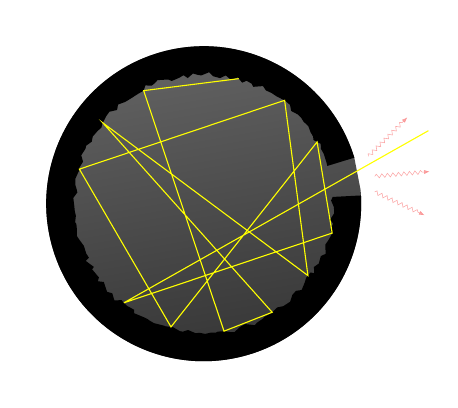
\begin{tikzpicture}[scale=2,rotate=10]
				  
				  \shade[top color=black!60,bottom color=black!80,shading angle=10] % background
				    (7:1) arc (7:355:1);
				  
				  \fill[thick,black,postaction=decorate, % rough inner surface
				    decoration={markings,mark=between positions 0.55 and 1 step 0.03 with {
				                  \node[transform shape,inner sep=1pt]
				                  (hit\pgfkeysvalueof{/pgf/decoration/mark info/sequence number}) {};
				    }}]
				    (7:1) arc (7:353:1) --++ (-7:-0.18)
				    decorate[decoration={random steps,segment length=2,amplitude=1pt}]
				        {arc (-7:-353:0.82)} -- cycle;
				  
				  \draw[yellow] % connect light ray to random points
				    (8:1.5) -- (hit6.center) -- (hit1.center) -- (hit15.center) -- (hit5.center) --
				    (hit9.center) -- (hit14.center) -- (hit2.center) -- (hit10.center) -- (hit3.center) --
				    (hit4.center) -- (hit11.center) -- (hit13.center);
				  
				  \foreach \ang in {-35,-5,35}{
				    \draw[radiation] (1,0)++(\ang:0.1 and 0.2) --++ (\ang:0.35);
				  }
				
				\end{tikzpicture}
				
					\caption{The Ideal Black Body Radiating after Receiving In-Falling Light (One Photon).}
					\label{fig:ideal_black_body_radiating_w_light}
			\end{figure}
			
			
			\begin{figure}[!ht]
				\centering
				% BLACK BODY - without infalling light
				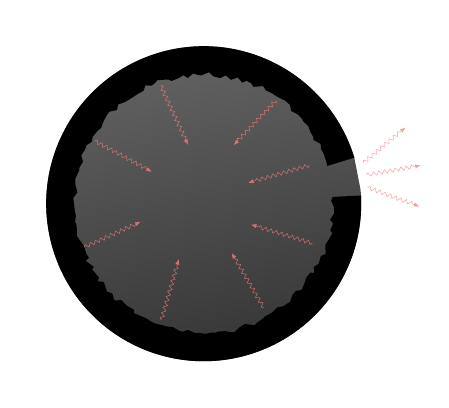
\begin{tikzpicture}[scale=2,rotate=10]
				  
				  \shade[top color=black!60,bottom color=black!80,shading angle=10] % background
				    (7:1) arc (7:355:1);
				  
				  \fill[thick,black,postaction=decorate, % rough inner surface
				    decoration={markings,mark=between positions 0.55 and 1 step 0.03 with {
				                  \node[transform shape,inner sep=1pt]
				                  (hit\pgfkeysvalueof{/pgf/decoration/mark info/sequence number}) {};
				    }}]
				    (7:1) arc (7:353:1) --++ (-7:-0.18)
				    decorate[decoration={random steps,segment length=2,amplitude=1pt}]
				        {arc (-7:-353:0.82)} -- cycle;
				  
				  \foreach \ang [evaluate={\angin=\ang-180+10*rand; \r=0.76+0.05*rand; \l=0.4+0.02*rand}] in {10,45,100,140,190,240,290,330}{
				    \draw[radiation] (\ang:\r) --++ (\angin:\l);
				  }
				  
				  \foreach \ang in {-30,0,30}{
				    \draw[radiation] (1,0)++(\ang:0.05 and 0.16) --++ (\ang:0.35);
				  }
				
				\end{tikzpicture}
				
				\caption{The Ideal Black Body still Radiating without In-Falling Light.}
				\label{fig:ideal_black_body_radiating_wout_light}
			\end{figure}
			
		\end{paracol}
		\vspace{10mm}
		
		\pagebreak
		
		It is said that Planck's mentor (in a story that must have occurred a hundred times before in science) told him it was not possible to describe the black body phenomena and that the limits of science had been reached. He ultimately revolutionised this field of study, based on the experimental results observed by others he formulated Planck's Law for black body radiation, given by Equation \ref{eqn:plancks_law_black_body}.\linebreak
		
		\columnratio{0.4}
		\begin{paracol}{2}
			
			\begin{equation}
				\mathlarger{\mathlarger{q_{\lambda} = \frac{2\pi c^2 h \lambda^{-5}}{e^{\frac{ch}{k_B \lambda T}}-1}}}
				\label{eqn:plancks_law_black_body}
			\end{equation}
			
		\switchcolumn
			
			\vspace{-10mm}
			\begin{align*}
				\text{Where:}& \\
					\lambda &= \text{Wavelength} \\
					k_B &= \text{Boltzmann's Constant} \\
					c &= \text{Celerity, Speed of Light in a Vacuum} \\
					q_{\lambda} &= \text{Energy Flux} \\
					\Planckconst &= \text{Planck's Constant} \\
					T &= \text{Temperature}
			\end{align*}
			
		\end{paracol}
			
		This equation perfectly described the emission curve of a black body based on temperature, shown below in Figure \ref{fig:curve_black_body_radiation}. Planck had unwittingly stumbled upon the basis of one of the most incredible fields of study in physics, and arguably one of the most important. He would go on to use this to develop quantum theory and the rest is history! \linebreak
		
		
		%%%% https://tikz.net/blackbody_plots/ %%%%
		\begin{figure}[!h]
			\centering
			% BLACK BODY - 3000, 4000, 5000K
			\begin{tikzpicture}
			  \message{^^JBlack body}
			  \def\N{60}
			  \def\xmax{3100}
			  \def\ymax{1.32e10}
			  \def\tick#1#2{\draw[thick] (#1+.01*\ymax) -- (#1-.01*\ymax) node[below=-.5pt,scale=0.75] {#2};}
			  \begin{axis}[
			      every axis plot/.style={
			        mark=none,samples=\N,domain=5:\xmax,smooth},
			      xmin=(-.05*\xmax), xmax=(1.05*\xmax),
			      ymin=(-.08*\ymax), ymax=(1.08*\ymax),
			      restrict y to domain=0:\ymax,
			      axis lines=middle,
			      axis line style=thick,
			      %enlargelimits=upper, % extend the axes a bit to the right and top
			      tick style={black,thick},
			      ticklabel style={scale=0.8},
			      %xtick style={draw=none},xticklabels=none,
			      xlabel={Wavelength $\lambda$ [nm]},
			      ylabel={Power $P$ [kW/sr\,m$^2$\,nm]},
			      xlabel style={at={(rel axis cs:0.5,0)},below=-1pt,font=\small},
			      ylabel style={at={(rel axis cs:-0.1,0.5)},rotate=90},
			      width=9cm, height=7cm,
			      %clip=false
			      tick scale binop=\times,
			      every y tick scale label/.style={at={(rel axis cs:0,1)},anchor=south}]
			    ]
			    
			    % RAINBOW
			    \shade[shading=rainbow,shading angle=90,opacity=0.5] (380,0) rectangle (740,\ymax);
			    \node[above=-1pt,scale=0.8] at (200,\ymax) {\strut UV}; % 10 - 400 nm
			    \node[above=-1pt,scale=0.8] at (570,\ymax) {\strut optical}; % 380 - 740 nm
			    \node[above=-1pt,scale=0.8] at (920,\ymax) {\strut IR}; % 740 - 1050 nm
			    
			    % PLANCK
			    \addplot[very thick,red]    {planck(x,3000)};
			    \addplot[very thick,orange] {planck(x,4000)};
			    \addplot[very thick,samples=3*\N,blue] {planck(x,5000)};
			    %\addplot[dashed,thick,red,domain=1000:4000]    {rayleighjeans(x,3000)};
			    %\addplot[dashed,thick,orange,domain=1000:4000] {rayleighjeans(x,4000)};
			    \addplot[dashed,thick,blue,domain=1000:4000]   {rayleighjeans(x,5000)};
			    %\addplot[dashed,thick,red,domain=1000:4000]    {wien(x,3000)};
			    %\addplot[dashed,thick,orange,domain=1000:4000] {wien(x,4000)};
			    %\addplot[dashed,thick,blue,domain=1000:4000]   {wien(x,5000)};
			    
			    %% MAXIMUM (Wien's displacement law)
			    %\addplot[mygreen,very thin,variable=T,domain=2500:6000]
			    %  ({lampeak(T)},{planck(lampeak(T),T)});
			    
			    % LABELS
			    \node[above=0pt,scale=0.75,red] at (1150,{planck(1150,3000)}) {\SI{3000}{K}};
			    \node[above right=-1pt,scale=0.75,orange!80!black] at (740,{planck(740,4000)}) {\SI{4000}{K}};
			    \node[above right=-1pt,scale=0.75,blue] at (800,{planck(800,5000)}) {\SI{5000}{K}};
			    \node[above right=-1pt,scale=0.75,blue] at (1500,{rayleighjeans(1500,5000)}) {\SI{5000}{K} Rayleigh-Jeans};
			    
			    %% TICKS
			    %\tick{500,0}{500}
			    %\tick{1000,0}{1000}
			    %\tick{1500,0}{1500}
			    %\tick{2000,0}{2000}
			    %\tick{2500,0}{2500}
			    %\tick{3000,0}{3000}
			    
			  \end{axis}
			\end{tikzpicture}
			
			\caption{Black Body Radiation Curve at Different Temperatures, the Classical Model (Rayleigh-Jones Curve) is Marked with a Dashed Line.}
			\label{fig:curve_black_body_radiation}
		\end{figure}
		
		
		\pagebreak
	
	
	
	
\section{The Photoelectric Effect}
	In 1905 Albert Einstein would use the findings of Planck's papers to finally describe the results of an experiment which had, until then, not been fully understood. The resulting effect was named the ``Photoelectric Effect''  \cite{wiki_photoelectric_effect}, it states ``that electrons are emitted when electromagnetic radiation, such as light, hits a material''. Electrons emitted in this way are known as ``Photoelectrons'' and this discovery was another key step in the development of quantum theory. It still finds uses in practical applications for chemistry and solid-state electronics today. \linebreak
	
	
	\subsection{The Photoelectric Experiment}
	The diagram of the photoelectric experiment is shown in Figure \ref{fig:photoelectric_effect_experiment_low_freq}, it consists of an ammeter, controlled DC voltage source, a collector, a photocathode, and a light source emitting monochromatic light.\linebreak
	If the DC voltage is kept constant and lower frequency light, of frequency $\nu_1$, is emitted towards the photocathode (as in Figure \ref{fig:photoelectric_effect_experiment_low_freq}) there is no current measured at the ammeter, no mater how long the light is shone or how intensely. \linebreak 
	However if light of a higher frequency, $\nu_2$, is shone at the photocathode (as in Figure \ref{fig:photoelectric_effect_experiment_high_freq}), the ammeter begins to immediately show current! \linebreak
	
	\begin{figure}[!h]
	\centering
	%%%% https://tikz.net/photoelectric_effect/ %%%%
		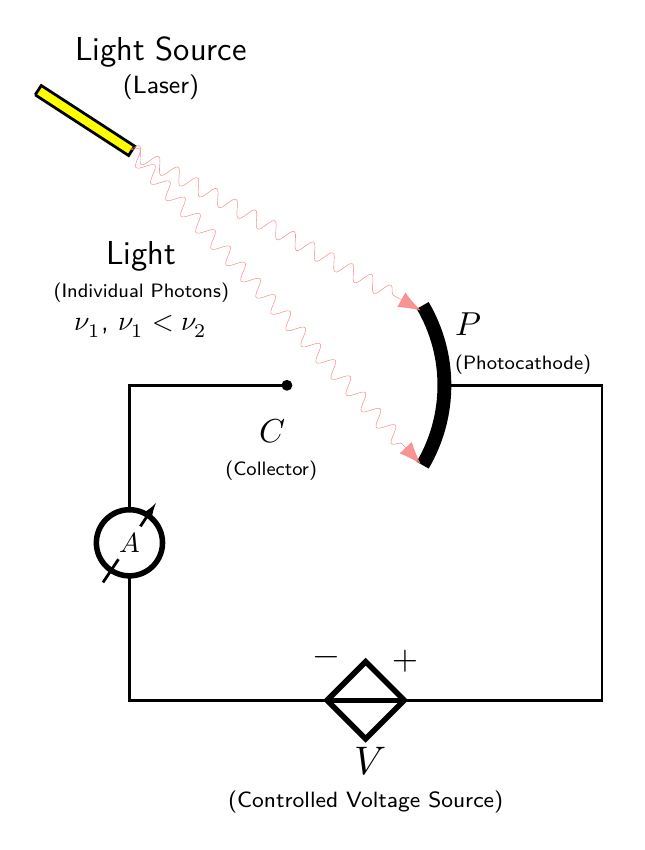
\begin{tikzpicture}[scale=1, line width=1]
			% Grid
%				\draw[help lines] (0,0) grid (11,11);
			
			% Circuits		
			\draw (4,6) -- (2,6) to[rmeterwa, t=$A$] ++(0,-4) -- (2,2) to[controlled voltage source, l_={
				\begin{tabular}{c}
					\Large $V$ \\
					\footnotesize (Controlled Voltage Source)
				\end{tabular}}] ++(6,0) -- (8,6) -- (6,6);
			\filldraw (4,6) circle [radius=0.05];
			
			% Dashed Arrows
			\draw[color=green!90,opacity=0,dashed,<-] (4,6) -- +(1.7,1)coordinate(A);
			\draw[color=green!90,opacity=0,dashed,<-] (4,6)coordinate(B) -- +(1.7,-1)coordinate(C);
			
			% Arc		
			\pic [draw, angle radius = 2cm, line width = 5] {angle=C--B--A};
			
			% Photocell
			\draw[color=black, line width=5, opacity=0] (5,6) circle [radius=1.8];
			
			% Laser
			\draw[fill=yellow, line width=1, rotate=12] (2.8,9.31) -- ++(1,-1) -- ++(0.1,0.1) -- ++(-1,1) -- +(-0.1,-0.1);
			%% Rays
			\draw[bigphoton] (2,9) -- (5.7,5);
			\draw[bigphoton] (2,9) -- (5.7,6.95);
			
			
			% Nodes
			\node at (5.5,2.5) {\large $+$};
			\node at (4.5,2.5) {\large $-$};
			\node at (3.8,5.15) {
				\begin{tabular}{c}
					\large $C$ \\
					\scriptsize (Collector)
				\end{tabular}};
			\node at (7,6.5) {
				\begin{tabular}{l}
					\large $P$ \\
					\scriptsize (Photocathode)
				\end{tabular}};
			\node at (2.4,10) {
				\begin{tabular}{c}
					\large Light Source \\
					\small (Laser)
				\end{tabular}};
			\node at (2.15,7.2) {
				\begin{tabular}{c}
					\large Light \\
					\scriptsize (Individual Photons) \\
					\normalsize $ \nu_1 $, $\nu_1 < \nu_2$
				\end{tabular}};
		\end{tikzpicture}
		
		\caption{A Diagram of the Photoelectric Experiment. Lower frequency light is being emitted and there is no activity in the experiment.}
		\label{fig:photoelectric_effect_experiment_low_freq}
	\end{figure}
	
	
	\pagebreak
	
	
	\begin{figure}[!h]
	\centering
	%%%% https://tikz.net/photoelectric_effect/ %%%%
		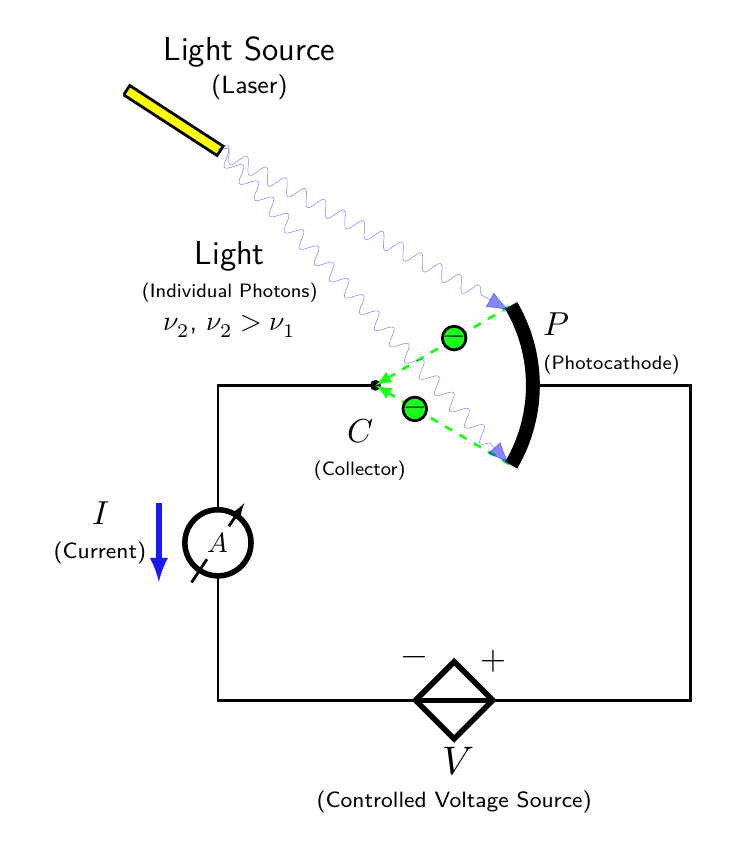
\begin{tikzpicture}[scale=1, line width=1]
%			% Grid
%				\draw[help lines] (0,0) grid (11,11);
			
			% Circuits		
			\draw (4,6) -- (2,6) to[rmeterwa, t=$A$] ++(0,-4) -- (2,2) to[controlled voltage source, l_={
				\begin{tabular}{c}
					\Large $V$ \\
					\footnotesize (Controlled Voltage Source)
				\end{tabular}}] ++(6,0) -- (8,6) -- (6,6);
			\filldraw (4,6) circle [radius=0.05];
			
			% Dashed Arrows
			\draw[color=green!90,dashed,<-] (4,6) -- +(1.7,1)coordinate(A);
			\draw[color=green!90,dashed,<-] (4,6)coordinate(B) -- +(1.7,-1)coordinate(C);
			
			% Arc		
			\pic [draw, angle radius = 2cm, line width = 5] {angle=C--B--A};
			
			% Photocell
			\draw[color=black, line width=5, opacity=0] (5,6) circle [radius=1.8];
			
			% Laser
			\draw[fill=yellow, line width=1, rotate=12] (2.8,9.31) -- ++(1,-1) -- ++(0.1,0.1) -- ++(-1,1) -- +(-0.1,-0.1);
			%% Rays
			\draw[bigphoton,color=blue!95,opacity=0.5] (2,9) -- (5.7,5);
			\draw[bigphoton,color=blue!95,opacity=0.5] (2,9) -- (5.7,6.95);
			
			% Electrons				
			\draw[fill=green!90] (4.5,5.7) circle [radius = 0.15];
			\draw[fill=green!90] (5,6.6) circle [radius = 0.15];
			%% Minus Symbol
			\node at (5,6.575) {$\symbf{-}$};
			\node at (4.5,5.675) {$\symbf{-}$};
			
			% Current
			\draw[blue!90, ->, line width = 2] (1.25,4.5) -- +(0,-1);
			
			% Nodes
			\node at (5.5,2.5) {\large $+$};
			\node at (4.5,2.5) {\large $-$};
			\node at (0.5,4.1) {
				\begin{tabular}{c}
					\large $I$ \\
					\footnotesize (Current)
				\end{tabular}};
			\node at (3.8,5.15) {
				\begin{tabular}{c}
					\large $C$ \\
					\scriptsize (Collector)
				\end{tabular}};
			\node at (7,6.5) {
				\begin{tabular}{l}
					\large $P$ \\
					\scriptsize (Photocathode)
				\end{tabular}};
			\node at (2.4,10) {
				\begin{tabular}{c}
					\large Light Source \\
					\small (Laser)
				\end{tabular}};
			\node at (2.15,7.2) {
				\begin{tabular}{c}
					\large Light \\
					\scriptsize (Individual Photons) \\
					\normalsize $ \nu_2 $, $\nu_2 > \nu_1$
				\end{tabular}};
		\end{tikzpicture}
		
		\caption{A Diagram of the Photoelectric Experiment. Higher frequency light is being emitted and electrons are passing across to the collector, and current is measured at the ammeter.}
		\label{fig:photoelectric_effect_experiment_high_freq}
	\end{figure}
	
	
	The experimental results described by the photoelectric effect inherently disagree with, and were unexplained by, classical electromagnetics which predicts that \textit{continuous} light waves transfer energy to electrons, which would then be emitted when they accumulate enough energy. An alteration in the intensity of light would theoretically (according to classical EM) change the kinetic energy of the emitted electrons, with sufficiently dim light resulting in a delayed emission. The experimental results instead showed that electrons are dislodged \textbf{only} when the light exceeds a certain frequency - regardless of the light's intensity or duration of exposure. \linebreak
	
	Another thing to note here is that, if we wished, we could increase the potential of the DC voltage source the flow of electrons would eventually stop again, and a higher frequency would be required to cause the transport of electrons across the gap. \linebreak
	

	\pagebreak
	
	\subsection{The Photoelectric Equation}
	So, as previously stated, in 1905 Albert Einstein used the findings of Planck to finally describe the results of the photoelectric experiment. He made an approximation, and stated the one quanta is absorbed by one electron (this is an approximation that he made to simplify his calculations, it is not true in every case). Then he stated that before the quanta is absorbed by the electron it's total energy is given by Equation \ref{eqn:photoelectric_1}. This is a simple, linear equation, rearranged in eq. \ref{eqn:photoelectric_2} it states what the \textit{kinetic} energy of the quanta is before interacting with the electron.  \linebreak
	
	
	\medskip
	
	
		\columnratio{0.4}
		\begin{paracol}{2}
			
			\begin{gather}
				\label{eqn:photoelectric_1} \mathlarger{\mathlarger{\Planckconst \nu = E_k + \Phi}} \\
				\label{eqn:photoelectric_2} \mathlarger{\mathlarger{E_k = \Planckconst \nu - \Phi}}
			\end{gather}
			
		\switchcolumn
			
			\vspace{-10mm}
			\begin{align*}
				\text{Where:}& \\
					E_k &= \text{Kinetic Energy} \\
					\Phi &= \text{Potential Energy (work function)} \\
					\nu &= \text{Frequency} \\
					\Planckconst &= \text{Planck's Constant}
			\end{align*}
		\end{paracol}
	
	\columnratio{0.7}
	\begin{paracol}{2}
		Equation \ref{eqn:photoelectric_2} provides a clearer explanation for why we were not propagating any photons across the gap when the frequency of the light was too low, we had to be over a threshold frequency, $\nu_{th}$, in order to overcome the potential! \linebreak
		Figure \ref{fig:photoelectric_effect_threshold} shows this rather simple relationship. There are also some other insights to be gleamed here, namely, that $E_K$ cannot be negative, that the work function is clearly material dependent, and that we can state a relationship to calculate the threshold frequency, given in Equation \ref{eqn:photoelectric_th}:
	
	\switchcolumn
		%% Kinetic energy - linear
		\begin{figure}[!h]
			\centering
			%%%% https://tikz.net/function_average/ %%%%
			\def\xmax{2.2} % max x axis
			\def\ymax{1.6} % max y axis
			\begin{tikzpicture}
				\message{^^JLinear}
				\def\a{0.17*\xmax}  % first limit
				\def\b{0.76*\xmax}  % last limit
				\def\k{\ymax/\xmax} % slope coefficient
							
				\draw[->,thick] (0,-0.15*\ymax) -- (0,\ymax+0.1) node[left] {$E_k$}; % y axis
				
				\draw[->,thick] (-0.15*\ymax,0) -- (\xmax+0.1,0) node[right=1,below] {$\nu$}; % x axis
				
				\draw[xline,line cap=round]
					(\a,0) -- (0.9*\xmax,0.9*\k*\xmax);
				\tick{\a,0}{90} node[below=-2,scale=0.8] {\strut $\nu_{th}$};
			\end{tikzpicture}
			\caption{Something...}
			\label{fig:photoelectric_effect_threshold}
		\end{figure}
	\end{paracol}
	
	\begin{align}
		& \mathlarger{ \Planckconst \nu \geq 0 } \nonumber\\
		& \mathlarger{ \therefore \: \Planckconst \nu \geq \Phi } \nonumber\\
		& \mathlarger{ \implies \nu \geq \frac{\Phi}{\Planckconst} } \nonumber\\
		& \label{eqn:photoelectric_th} \mathlarger{ \therefore \: \nu_{th} = \frac{\Phi}{\Planckconst} }
	\end{align}
	
	Since we can also state the potential energy, $E_k$ in terms of charge and voltage, this means that we can obtain another equation (\ref{eqn:photoelectric_vstop}) to express $E_k$ based on the biasing voltage required to stop the electrons from flowing when particular frequencies of light are incident on the plates.
	
	\begin{align}
		& \mathlarger{ E_k = C \times V_{stop} } \nonumber\\
		& \label{eqn:photoelectric_vstop} \mathlarger{ \therefore \: E_k = e \times V_{stop} }
	\end{align}
	
		
	\subsection{A Quick Example}
		Let's (as a demonstrative example) calculate how many quanta we might have traveling in a given beam of light... \linebreak
		You probably know the meaning of flux quite well in classical electromagnetic theory (namely a vector quantity describing the magnitude and direction of the flow of electromagnetic energy). But we can (an probably must) redefine the meaning of flux with our new-found knowledge of quanta, considering the discrete definition of quanta instead of non-discrete EM energy, see Equation \ref{eqn:quantum_flux}: \linebreak
		
		\begin{equation}
			\label{eqn:quantum_flux} \mathlarger{\text{\normalsize Flux}, F = \frac{\text{\normalsize no. of quanta}, n}{\text{\normalsize area}, a \times \text{\normalsize time}, t}}
		\end{equation}
		
		\vspace{5mm}
		
		Given the definition of intensity, shown in \ref{eqn:intenisty_def}, let's say the intensity and wavelength of the light beam are $I=2w/m^2$ and $\lambda=250nm$ respectively. We'll begin by calculating the energy of one single quanta (Equation \ref{eqn:ex_1_energy_single_quant}), then we'll calculate the number of quanta emitted by our light beam (Equation \ref{eqn:ex_1_quant_in_beam}), and finally we could combine those two equations to get the total energy once given beam diameter (or area) and time. \linebreak
	
		\begin{align}
			& \text{Energy of a single quanta} \nonumber\\
			& \mathlarger{ E = \Planckconst \nu = \frac{\Planckconst c}{\lambda} = \frac{12.4 \times 10^3 eV \cdot \si{\angstrom}}{250 \times 10^{-9} m } \text{\hspace{5mm}\footnotesize Remember an Angstrom is $1 \times 10^{-10}$ metres}} \nonumber\\
			& \label{eqn:ex_1_energy_single_quant} \mathlarger{ \implies \text{\normalsize 1 Quanta } = 4.96\ eV} \\
			& \text{Number of quanta in the beam} \nonumber\\
			& \label{eqn:intenisty_def} \mathlarger{ \text{\small Intensity }= 2\ \frac{w}{m^2} = 2\ \frac{J}{m^2 \times s} } \\
			& \mathlarger{ \therefore \ \frac{N}{m^2s} = 2\ \frac{J}{m^2 \times s} \times \frac{1}{\Planckconst \nu} = 2\ \frac{J}{m^2 \times s} \times \frac{1}{4.96 \cdot 1.602 \times 10^{-19} J} } \nonumber\\
			& \label{eqn:ex_1_quant_in_beam} \mathlarger{ \text{\small   No. of Quanta /$m^2s$} \approx  2.52 \times 10^{18} }
		\end{align}
		
		
	\pagebreak
	
	
	
	
\section{Bohr’s Model of the Hydrogen Atom}
	
	\subsection{Bohr’s Hypothesis - Angular Momentum is Quantised}
		Bohr's hypothesis was that the angular momentum for small particles is quantised (along with a number of other properties) and that as a consequence this would result in a particular model or interpretation of the hydrogen atom. Explicitly, Bohr's hypothesis is derived below, then written in Equation \ref{eqn:bohrs_hypthesis}. \linebreak
		
		\begin{gather}
			\mathlarger{ \text{\small Classically, Angular Momentum would be } \int L_{\theta} \,d\theta = \Planckconst n } \nonumber\\
			\mathlarger{ \text{\small Bohr's Hypothesis } \implies \int L_{\theta} \,d\theta = L_{\theta} \oint^{2\pi}_0 \,d\theta = L_{\theta} \cdot 2 \pi } \nonumber\\ 
			\label{eqn:bohrs_hypthesis} \mathlarger{ \therefore \; L_{\theta} = \frac{\Planckconst}{2 \pi} n = \hbar n }
		\end{gather}
		
		\vspace{5mm}
		
		Thus, in quantum physics, the angular momentum is quantised and an integer multiple of Planck's reduced constant, $\hbar$. Now we will see the implications of this hypothesis and how this helped Bohr construct his model of the Hydrogen atom. \linebreak
		
		
	\subsection{Force Balance}
		In order to have electrons orbiting a central nucleus they must be under a ``centrifugal'' force. \linebreak
		
		\begin{equation*}
			\text{\small Force, }F = \text{mass, }m \cdot \frac{\text{\small Instant. Velocity, }V_R^2}{\text{\small radius, }r}
		\end{equation*}
		
		\vspace{5mm}
		
		As we assume the only attractive/repellent forces in play here must be electromotive, the centrifugal force must therefore be equal to the electromotive forces. Given our previous definitions regarding E.M.F we can state: \linebreak
		
		\begin{gather*}
			\text{\small Force, }F \; = \; \text{mass, }m \cdot \frac{\text{\small Instant. Velocity, }V_R^2}{\text{\small radius, }r} \; = \; \frac{e^2}{r^2} \\
			\\
			\therefore \;  r = \; \frac{e^2}{m \; V_R^2}
		\end{gather*}
		
		
	\subsection{Bohr’s Radius}
		
		
	\subsection{Velocity}
	
	
	\subsection{Energy an Energy Levels}
	
	
	\pagebreak
	
	
	
	
\section{The Wave Nature of Matter}
	
	\subsection{De Broglie and The De Broglie Wavelength}
	
	
	\subsection{Uses - Electron Microscope vs Conventional Light Microscope}
	
	
	\subsection{The Double Slit Experiment}
	
	
	\subsection{Augen’s Principle}
	
	
	\pagebreak
	
	
	
	
\section{Particle Interference}
	
	\subsection{The Double Slit Experiment Explored}
	
	
	\subsection{Possible Solutions}
	
	
	\subsection{Superposition of Solutions}
	
	
	\subsection{Final Solution}
	
	
	\subsection{Diffraction of Particles}
	
	
	\pagebreak
	
	
	
	
\section{The Schrödinger Equation}
	
	\subsection{The general Schrödinger Equation in time and space}
	
	
	\subsection{The Superposition Principle}
	
	
	\subsection{The S.E.’s Eigenfunction and its Properties}
	
	
	\subsection{The Wave function; its Properties and Conditions}
	
	
	\subsection{Possible Solutions to the Eigen and Wave functions}
	
	
	\subsection{The Kroncker Equation}
	
	
	\subsection{A particle with mass (m) moving in one dimension according to the S.E.}
	
	
	\pagebreak
	
	
	
	
\section{Observables}
	
	\subsection{What are Observables?}
	
	
	\subsection{Calculating Observables, Step-by-Step}
	
	
	\pagebreak
	
	
	
	
\section{Confinement}
	
	\subsection{Confined Particles in 1D}
		
		\subsubsection{The Quantum Well}
		
		
		\subsubsection{Using the S.E., Eigen, and Wave Functions to Find Solutions to observables}
		
		
		\subsubsection{Conditions}
		
		
		\subsubsection{Superposition of Solutions}
		
		
	\subsection{Hisenburg Principle}
	
	
	\subsection{Paul Exclusion Principle}
	
	
	\subsection{Confined Particles in 3D}
	
	
	\subsection{The Fermi Level}
	
	
	\subsection{Confined Particles in 1D - Realistic (Finite Potential) Boundaries}
	
		\subsubsection{Symmetric QW}
		
		
		\subsubsection{Asymmetric QW}
		
		
		\subsubsection{The Wave Vector}
		
		
		\subsubsection{Examples}
		
		
	\subsection{Quantum Tunneling}
	
		\subsubsection{General Example and Solution for Tunneling Across a 1D Boundary}
		
		
		\subsubsection{Electron Microscope}
		
		
	\subsection{Quantum Oscillators - Parabolic QW/Confinement}
	
	
	\pagebreak
	
	
	
	
\section{Periodic Photonic Structures}\vskip0pt
	{\quad\quad\color{heading}\ReportSectionFont{Block Modes in Periodic, Quantum Structures}}
		
	\subsection{The Transfer Matrix}
	
	
	\subsection{Applying the Transfer Matrix}
	
	
	\subsection{Block Theorem}
	
	
	\subsection{Solution Cases/Types for the Quantum Structure}
	
	
	\subsection{The Quantum Bandgap}
	
	
	\subsection{2D Periodic Structure for Electron Containment}
	
	
	\subsection{Time Reversal of the Transfer Matrix}
	
	
	\pagebreak
	
	
	
	
\section{Angular Momentum and Commutators}
	
	\subsection{Angular Momentum - Classical Perspectives}
	
	
	\subsection{Angular Momentum - Quantum Interpretation}
	
	
	\subsection{What is Commutation?}
	
	
	\subsection{Commutation Examples and Useful Results}
	
	
	\subsection{The Meaning of Commutation - Common Sets of Eigen Functions}
	
	
	\subsection{Energy Levels in the Presence of a Magnetic Field - The Zeeman Effect}
	
	
	\subsection{The Zeeman Effect and Free Angular Momentum}
	
	
	\subsection{Orbital Angular Momentum}
	
	
	\subsection{Orbital Angular Momentum - Quantisation}
	
	
	\pagebreak
	

\section{Some interesting Applications}
	
	\subsection{NMR - Nuclear Magnetic Resonance}
	
	\subsection{Quantum Bit}
		
	
	\subsection{Spontaneous Parametric Down Conversion}
	
	\subsection{No-Cloning Theorem}
	
	\subsection{Shor's Algorithm}
	
	
	
		
\section{Appendix}
	
	\subsection{Constants \& Relevant Definitions}
		
		\subsubsection{Constants}
		
			\begin{center}
				\color{body}
				\begin{longtblr}[
					caption = {\textit{Important constants involved in Quantum Mechanics}},
					label = {tab:important_constants_qm}
					]{
					colspec={|X[15,l,m]|X[28,l,m]|X[29,l,m]|},
					rows = {abovesep=2mm,belowsep=2mm}
					}
			    		\hline
					\textit{\textbf{Symbol/Definition}} & \textit{\textbf{Name/info}} & \textit{\textbf{Value}} \\ 
					\hline
					$\symbf{c}$ & \textit{Speed of Light in Vacuum} \cite{wiki_speed_of_light} & \textit{$2.998\times10^{8}$ metres/second (m/s)} \\ 
					\hline
					$\symbf{e}$ & \textit{Charge of an Electron} \cite{wiki_electron} & \textit{$-1.602\times10^{-19}$ Coulomb (C)} \\ 
					\hline
						\SetCell[r=2]{m} $\symbf{\Planckconst}$ & 
							\SetCell[r=2]{m} \textit{Planck's Constant} \cite{wiki_plancks_constant} & 
								\textit{$6.626\times10^{-34}$ Joule$\cdot$second (J$\cdot$s)} \\
						&& \textit{= $4.136\times10^{-15}$ eV$\cdot$second (eV$\cdot$s)}  \\
					\hline
						\SetCell[r=2]{m} $\pmb{\hbar}\symbf{=\frac{\Planckconst}{2\pi}}$ & 
							\SetCell[r=2]{m} \textit{The reduced Planck constant, Planck's constant in terms of Radians instead of Hertz.} \cite{wiki_plancks_reduced_constant} & 
								\textit{$1.055\times10^{-34}$ Joule$\cdot$second (J$\cdot$s)} \\
						&& \textit{= $0.658\times10^{-15}$ eV$\cdot$second (eV$\cdot$s)} \\ 
					\hline
					$\symbf{k_e=\frac{1}{4\pi\epsilon_0}}$ & \textit{Coulomb's Constant, the Electric Force Constant, or the Electrostatic Constant.} \cite{wiki_coulombs_constant} & \textit{$8.988\times10^9$ $\frac{\text{Newton$\cdot$metre$^2$}}{\text{Coulomb$^2$}}$ $ \left( \frac{\text{N$\cdot$m$^2$}}{\text{C$^2$}} \right) $} \\ 
					\hline
					$\symbf{N_A}$ & \textit{Avogadro's Constant} \cite{wiki_avogadros_constant} & \textit{$6.022\times10^{23}$ mole$^{-1}$ or $\frac{1}{\text{mole}}$} \\
					\hline
						\SetCell[r=2]{m} $\symbf{G}$ & 
							\SetCell[r=2]{m} \textit{Gravitational Constant} \cite{wiki_gravitational_constant} & 
								\textit{$6.672 \times 10^{-11}$ $\frac{\text{metre$^3$}}{\text{Kilogram$\cdot$second$^2$}}$ $\left(\frac{\text{m$^3$}}{\text{Kg$\cdot$s$^2$}}\right)$} \\
						 & & \textit{= $6.672 \times 10^{-8}$ $\frac{\text{centimetre$^3$}}{\text{gram$\cdot$second$^2$}} $ $\left( \frac{\text{cm$^3$}}{\text{g$\cdot$s$^2$}}  \right) $} \\
					\hline
						$\symbf{k_B=\frac{R}{N_A}}$ & 
							\SetCell[r=2]{m} \textit{Boltzmann's Constant, this relates the relative kinetic energy of particles in a gas with the thermodynamic temperature of the gas.} \cite{wiki_boltzmann_constant} & 
								\textit{$1.38\times10^{-23}$ Joule$\cdot$Kelvin (J$\cdot$K)} \\
						\textit{$\left(\frac{\text{Molar Gas Constant}}{\textit{Number of Molecules}} \right)$} & & \textit{= $8.617\times10^{-5}$ eV$\cdot$Kelvin (eV$\cdot$K)} \\
					\hline
						\SetCell[r=3]{m} $\symbf{\Planckconst  c}$ & 
							\SetCell[r=3]{m} \textit{Planck's Constant $\cdot$ Speed of Light in Vacuum} & 
								\textit{$19.865\cdot10^{-26}$ Joules$\cdot$metre (J$\cdot$m)} \\
						 & & \textit{$12.41\cdot10^{3}$ electronvolt$\cdot$Angstrom (eV$\cdot$\r{A})} \\
						 & & \textit{$1241$ Mega-electronvolt$\cdot$femto-metre (MeV$\cdot$fm)} \\
					\hline
					\pagebreak
						\SetCell[r=3]{m} $\pmb{\hbar} \symbf{c}$ & 
							\SetCell[r=2]{m} \textit{Normalised Planck's Constant $\cdot$ Speed of Light in Vacuum} & 
								\textit{$3.165\cdot10^{-26}$ Joules$\cdot$metre (J$\cdot$m)} \\
						 & & \textit{$1973$ electronvolt$\cdot$Angstrom (eV$\cdot$\r{A})} \\
						 & & \textit{$197.3$ Mega-electronvolt$\cdot$femto-metre (MeV$\cdot$fm)} \\
					\hline
					$\symbf{k_ce^2}$ & \textit{Coulomb's Constant$\cdot$energy$^2$} & \textit{$1.44$ Mega-electronvolt$\cdot$femto-metre (MeV$\cdot$fm) } \\
					\hline
					$\symbf{\frac{k_ce^2}{\pmb{\hbar} \, c}}$ & \textit{The Fine-Structure Constant} \cite{wiki_fine_structure_constant} & $\frac{1}{137}$ \\
					\hline
						\SetCell[r=2]{m} $\symbf{{\mu}_B = \frac{e \, \pmb{\hbar}}{2 \, m_e}}$ & 
							\SetCell[r=2]{m} \textit{The Bohr Magneton} \cite{wiki_bohr_magneton} & 
								\textit{$9.27\times10^{-24}$ Joule/Tesla (J/T) } \\
						 & & \textit{$5.79\times10^{-5}$ electronvolt/Tesla (eV/T) } \\	
					\hline
			    \end{longtblr}
			\end{center}
		
		
		\subsubsection{Relevant Classical Definitions}
			TODO
			
			\begin{table}[h!]
				\color{body}
				\SetTblrInner{rowsep=2.5mm}
				\begin{tblr}{colspec={|X[c,m]|X[c,m]|}}
			    		\hline
					Force Moving on a Charge & Electric Field of a Charge \\
					\hline
					Magnetic Field of a Current & Induced Electromotive Force \\
					\hline
					\SetCell[c=2]{c} Energy Density in the Field \\
					\hline
				\end{tblr}
				\caption{\label{tab:important_definitions_qm}\textit{Important Definitions Involved in Classical Physics that will be Relevant for Quantum Physics.}}
			\end{table}
			
			
			
			\pagebreak
	
	
	
	
	\subsection{Units Involved and Some Important Starting Equations}
		
		
		\begin{center}
		\color{body}
			\begin{longtblr}[
				caption = {\textit{Important Units Involved in Classical Physics that will be Relevant for Quantum Physics.}},
				label = {tab:important_units_qm}
				]{
				colspec={|X[28,l,m]|X[10,c,m]|X[28,l,m]|},
				rows = {abovesep=2mm,belowsep=2mm},
				vline{1,4} = {5}{white},
				vline{1,4} = {11}{white},
				vline{1,4} = {16}{white},
				vline{1,4} = {21}{white},
				vline{1,4} = {25}{white},
				}
				\hline
				\textit{\textbf{Measurement/Info}} & \textit{\textbf{Abbreviation}} & \textit{\textbf{SI Unit (\& Other Common/Useful Units)}} \\
				\hline
				Distance & $s$ & \textit{metres (m)} \\
				\hline
				Mass & $m$ & \textit{kilograms (kg)} \\
				\hline
				Time & $t$ & \textit{second (s)} \\
				\hline
					\SetCell[c=3]{m} \\ %% 5
				\hline
				Velocity & $v$ & \textit{metres/Second (m/s)} \\
				\hline
				Momentum & $p$ & \textit{$\frac{\text{kilogram$\cdot$metres}}{\text{second}}$ $\left(\frac{\text{kg$\cdot$m}}{\text{s}}\right)$} \\
				\hline
				Force & $F$ & \textit{Newtons (N), $\frac{\text{kilogram$\cdot$metres}}{\text{second$^2$}}$ $\left(\frac{\text{kg$\cdot$m}}{\text{s$^2$}}\right)$} \\
				\hline
				Energy, Work Done & $W, \,E$ & \textit{Joules (J), Newton metres (Nm)} \\
				\hline
				Power & $P$ & \textit{Watts (W), $\frac{\text{Joules}}{\text{second}}$ $\left(\frac{\text{J}}{\text{s}}\right)$} \\
				\hline
					\SetCell[c=3]{m} \\ %% 11
				\hline
				Electric Charge & $q$ & \textit{Coulombs (C), Ampere$\cdot$seconds (A$\cdot$s)} \\		
				\hline
				Electric Charge Density & $\rho$ & \textit{$\frac{\text{Coulomb}}{\text{metre$^3$}}$ $\left( \frac{\text{C}}{\text{m}^3} \right)$} \\
				\hline
				Electric Potential & $\varphi$ & \textit{Volts (V), $\frac{\text{Joules}}{\text{Coulomb}}$ $\left( \frac{\text{J}}{\text{C}} \right)$} \\		
				\hline
				Electric Field & $\vec{E}$ & \textit{$\frac{\text{Volts}}{\text{metre}}$ $\left( \frac{\text{V}}{\text{m}} \right)$, $\frac{\text{Newtons}}{\text{Coulomb}}$ $\left( \frac{\text{N}}{\text{C}} \right)$} \\
				\hline
					\SetCell[c=3]{m} \\ %% 16
				\hline
				Electric Current & $I$ & \textit{Amperes (A), $\frac{\text{Coulomb}}{\text{second}}$ $\left( \frac{\text{C}}{\text{s}} \right)$} \\
				\hline
				Electric Current Density & $\vec{J}$ & \textit{$\frac{\text{Amperes}}{\text{metre$^2$}}$ $\left( \frac{\text{A}}{\text{m}^2} \right)$} \\
				\hline
				\pagebreak
				Resistance & $R$ & \textit{Ohm ($\Omega$), $\frac{\text{Volts}}{\text{Ampere}}$ $\left( \frac{\text{V}}{\text{A}} \right)$} \\
				\hline
				Resistivity & $\rho$ & \textit{Ohm$\cdot$metre ($\Omega \cdot$m)} \\
				\hline
					\SetCell[c=3]{m} \\  %% 21
				\hline
				Magnetic Flux Density & $\vec{B}$ & \textit{Tesla (T), $\frac{\text{Newtons}}{\text{Ampere$\cdot$metre}}$ $\left( \frac{\text{N}}{\text{A$\cdot$m}} \right)$} \\
				\hline
				Magnetic Field Strength & $\vec{H}$ & \textit{$\frac{\text{Amperes}}{\text{metre}}$ $\left( \frac{\text{A}}{\text{m}} \right)$} \\
				\hline
				Magnetic Flux & $\vec{\Phi}$ & \textit{Weber (W), Tesla$\cdot$metre$^2$ (T$\cdot$m$^2$)} \\
				\hline
					\SetCell[c=3]{m} \\ %% 25
				\hline
				Capacitance & $C$ & \textit{Farads (F), $\frac{\text{seconds}}{\text{Ohm}}$ $\left( \frac{\text{s}}{\Omega} \right)$} \\
				\hline
				Inductance & $L$ & \textit{Henries (H), Ohm$\cdot$seconds ($\Omega\cdot$s)} \\
				\hline
 		    \end{longtblr}
		\end{center}
		
		
		\bigskip
	
	
	
	
	\subsection{Conversions}
		
		\begin{table}[h!]
			\color{body}
			\centering
			\SetTblrInner{rowsep=2.5mm}
			\begin{tblr}{width=12cm,colspec={|X[1,l,m]|X[1,l,m]|}}
			    	\hline
				$1$ electronvolt (eV) & $1.602\times10^{-19}$ Joules (J) \\	
				\hline
				$1$ Angstrom (\r{A}) & $10\times10^{-10}$ metres (m) \\
				\hline
				$1$ Ohm ($\Omega$) & $1.13\times10^{-12}$ $\frac{\text{seconds}}{\text{centimetre}}$ $\left( \frac{\text{s}}{\text{cm}} \right)$ \\
				\hline
				$1$ Farad (F) & $9\times10^{8}$ metres (m) \\
				\hline
				$1$ Henry (H) & $1.13\times10^{-12}$ $\frac{\text{seconds}^2}{\text{centimetre}}$ $\left( \frac{\text{s}^2}{\text{cm}} \right)$ \\
				\hline
			\end{tblr}
			\caption{\label{tab:important_conversions_qm}\textit{Some Conversions for Quantum Mechanics}}
		\end{table}
		
		
		
		
		\pagebreak
	
	
	
	
	
	\subsection{Properties of Elemental Particles}
		
		\begin{table}[h!]
			\color{body}
			\centering
			\SetTblrInner{rowsep=2.5mm}
			\begin{tblr}{width=12cm,colspec={|X[24,l,m]|X[12,l,m]|X[28,l,m]|}}
				\hline
				    	\SetCell[c=3]{c} {\color{subheading}\ReportSubSectionFont{Electron Properties}} \cite{wiki_electron} \\
			    	\hline
				\textit{\textbf{Property}} & \textit{\textbf{Abbreviation}} & \textit{\textbf{Value}} \\ 
				\hline
					\SetCell[r=2]{m} \textit{Mass at rest} & 
						\SetCell[r=2]{m} $\symbf{m_{e}}$ & 
							\textit{$9.109\times10^{-31}$ kilogram (kg)} \\ 
					& & \textit{$9.109\times10^{-28}$ gram (g)} \\
				\hline
					\SetCell[r=2]{m} \textit{Charge} & 
						\SetCell[r=2]{m} $\symbf{q_{e}}$, $\symbf{e^-}$ & 
							\textit{$−1$ elementary charge (e)} \\ 
					& & \textit{$−1.602\times10^{-19}$ Coulombs (C)} \\
				\hline
				\textit{Energy} & $\symbf{E_{e} = m_ec^2}$ & \textit{$0.511$ Mega electronvolt (MeV)} \\ 
				\hline
					\SetCell[r=2]{m} \textit{Intrinsic Magnetic Moment} & 
						\SetCell[r=2]{m} $\symbf{\mu_{e}}$ & 
							\textit{$−9.285\times10^{-24}$ Joule/Tesla (J/T)} \\
					& & $−1.001$ Bohr Magneton ($\mu_B$) \\
				\hline
				\textit{Spin} & $\symbf{S_{e}}$ & \textit{$\pm\frac{1}{2}$} \\	
				\hline
			\end{tblr}
			\caption{\label{tab:electron_properties_qm}\textit{Important Properties of the Electron for Quantum Mechanics}}
		\end{table}
		
		
		\bigskip
		
		
		\begin{table}[h!]
			\color{body}
			\centering
			\SetTblrInner{rowsep=2.5mm}
			\begin{tblr}{width=12cm,colspec={|X[24,l,m]|X[12,l,m]|X[28,l,m]|}}
			    	\hline
				    	\SetCell[c=3]{c} {\color{subheading}\ReportSubSectionFont{Proton Properties}} \cite{wiki_proton} \\
			    	\hline
				\textit{\textbf{Property}} & \textit{\textbf{Abbreviation}} & \textit{\textbf{Value}} \\ 
				\hline
					\SetCell[r=2]{m} \textit{Mass at rest} & 
						\SetCell[r=2]{m} $\symbf{m_{p}}$ & 
							\textit{$1.673\times10^{-27}$ kilogram (kg)} \\ 
					& & \textit{$1.673\times10^{-24}$ gram (g)} \\
				\hline
					\SetCell[r=2]{m} \textit{Charge} & 
						\SetCell[r=2]{m} $\symbf{q_p}$, $\symbf{e^+}$ & 
							\textit{$+1$ elementary charge (e)} \\ 
					& & \textit{$+1.602\times10^{-19}$ Coulombs (C)} \\
				\hline
				\textit{Energy} & $\symbf{E_p = m_pc^2}$ & \textit{$938.3$ Mega electronvolt (MeV)} \\ 
				\hline
					\SetCell[r=2]{m} \textit{Intrinsic Magnetic Moment} & 
						\SetCell[r=2]{m} $\symbf{\mu_p}$ & 
							\textit{$+1.411\times10^{-26}$ Joule/Tesla (J/T)} \\
					& & $+1.521\times10^{-3}$ Bohr Magneton ($\mu_B$) \\
				\hline
				\textit{Spin} & $\symbf{S_p}$ & \textit{$\pm\frac{1}{2}$} \\	
				\hline
			\end{tblr}
			\caption{\label{tab:proton_properties_qm}\textit{Important Properties of the Proton for Quantum Mechanics}}
		\end{table}
		
		
		\pagebreak
		
		
		{\color{subheading}\ReportSubSectionFont{Properties of Elemental Particles Cont...}}
		
		\bigskip
		
		
		\begin{table}[h!]
			\color{body}
			\centering
			\SetTblrInner{rowsep=2.5mm}
			\begin{tblr}{width=12cm,colspec={|X[24,l,m]|X[12,l,m]|X[28,l,m]|}}
			    	\hline
					\SetCell[c=3]{c} {\color{subheading}\ReportSubSectionFont{Neutron Properties}} \cite{wiki_neutron} \\
				\hline
				\textit{\textbf{Property}} & \textit{\textbf{Abbreviation}} & \textit{\textbf{Value}} \\ 
				\hline
					\SetCell[r=2]{m} \textit{Mass at rest} & 
						\SetCell[r=2]{m} $\symbf{m_{n}}$ & 
							\textit{$1.675\times10^{-27}$ kilogram (kg)} \\ 
					& & \textit{$1.675\times10^{-24}$ gram (g)} \\
				\hline
					\SetCell[r=2]{m} \textit{Charge} & 
						\SetCell[r=2]{m} $\symbf{q_n}$ & 
							\textit{$\approx 0$ elementary charge (e)} \\ 
					& & \textit{$(-2 \pm 8) \times 10^{-22}$ e} \\
				\hline
				\textit{Energy} & $\symbf{E_n = m_nc^2}$ & \textit{$939.6$ Mega electronvolt (MeV)} \\ 
				\hline
				\textit{Intrinsic Magnetic Moment} & $\symbf{\mu_n}$ & \textit{$\approx 0$ Joule/Tesla (J/T)} \\
				\hline
				\textit{Spin} & $\symbf{S_n}$ & \textit{$\pm\frac{1}{2}$} \\	
				\hline
			\end{tblr}
			\caption{\label{tab:neutron_properties_qm}\textit{Important Properties of the Neutron for Quantum Mechanics}}
		\end{table}
		
		
		\pagebreak
		
	
	
	
\newpage
\setstretch{1}  % Reduce bibliography line spacing
\bibliography{references.bib}
\bibliographystyle{IEEETran}
\end{document}
